\section{Self-Supervised Representation Learning}
\label{sec:ssl_contextualization}

% \fromsurvey{In a scenario where the efficacy of transfer learning via fine-tuning from pretrained supervised networks is limited due to geographical domain shift \citep{nyborg2022timematch}, more robust strategies are required, such as knowledge distillation \citep{bazzi2020distilling}, domain adaptation \citep{wang2021phenology} or self-supervised learning \citep{yuan2020self,yuan2022sits,xu2024self}. This is aggravated by the lack of vast labeled datasets (see Table \ref{tab:context_labeled_datasets}), which prompted research in the field of Deep Learning for \ac{RS} seems to move towards unsupervised representation learning. In this sense, Foundational Models (FMs) are one of the most prominent family of representational methods, capable of learning richer representations from multi-modal data, enabling zero-shot predictions on a variety of tasks. FMs seem better suited for remote sensing tasks due to the lack of labeled data \citep{huo2025remote}, but there are many challenges, including data acquisition, training efficiency, data shift, and practical application challenges to use FMs in real-world scenarios \citep{yin2025fms}.}

%\fromsurvey{As described by \citep{liu2021self}, the two most common ways of computing such representations directly from unlabeled data are: (i) generative modeling; and (ii) self-supervision. In the remaining sections of this manuscript, we focus on the latter approach and its application to agricultural tasks.}


\Acf{SSL} \fromsurvey{consists of extracting supervision signals from unlabeled data, usually widely available in \ac{RS}. These procedurally computed labels are then used for pretraining learning models, which can be fine-tuned for downstream tasks using smaller amounts of labeled data \citep{balestriero2023cookbookselfsupervisedlearning}. Several visual \ac{SSL} methods \citep{he2021maskedautoencodersscalablevision} are inspired by techniques used in the pretraining phases of \acs{LLM}s such as \ac{BERT} \citep{devlin2019bert}, wherein the model is trained to recover masked words from the context of neighboring words.}

It is well known in the literature that Transfer Learning between supervised trainings does not work very well for \ac{RS}, given that the models do not generalize well between different regions, especially in agriculture, since there are climatological, soil, and even subspecies differences, where the same crop class has different subspecies for each region. Furthermore, supervised datasets are scarce (as demonstrated in \autoref{tab:context_labeled_datasets}). Therefore, \ac{SSL} proves to be a particularly useful tool for agricultural \ac{RS}, considering all these problems described, in addition to the abundance of unlabeled data, since satellites are constantly acquiring data, and there are several publicly available missions (as demonstrated in \autoref{tab:context-satellites}), plus the main characteristic of \ac{SSL} of learning intrinsic features of the target data.

\newcommand{\figscale}{0.5}

\begin{figure}[ht!]
    \centering
    \caption{Overview of the self-supervised pretraining and finetuning process.}
    \begin{subfigure}[c]{0.975\columnwidth}
        \centering
        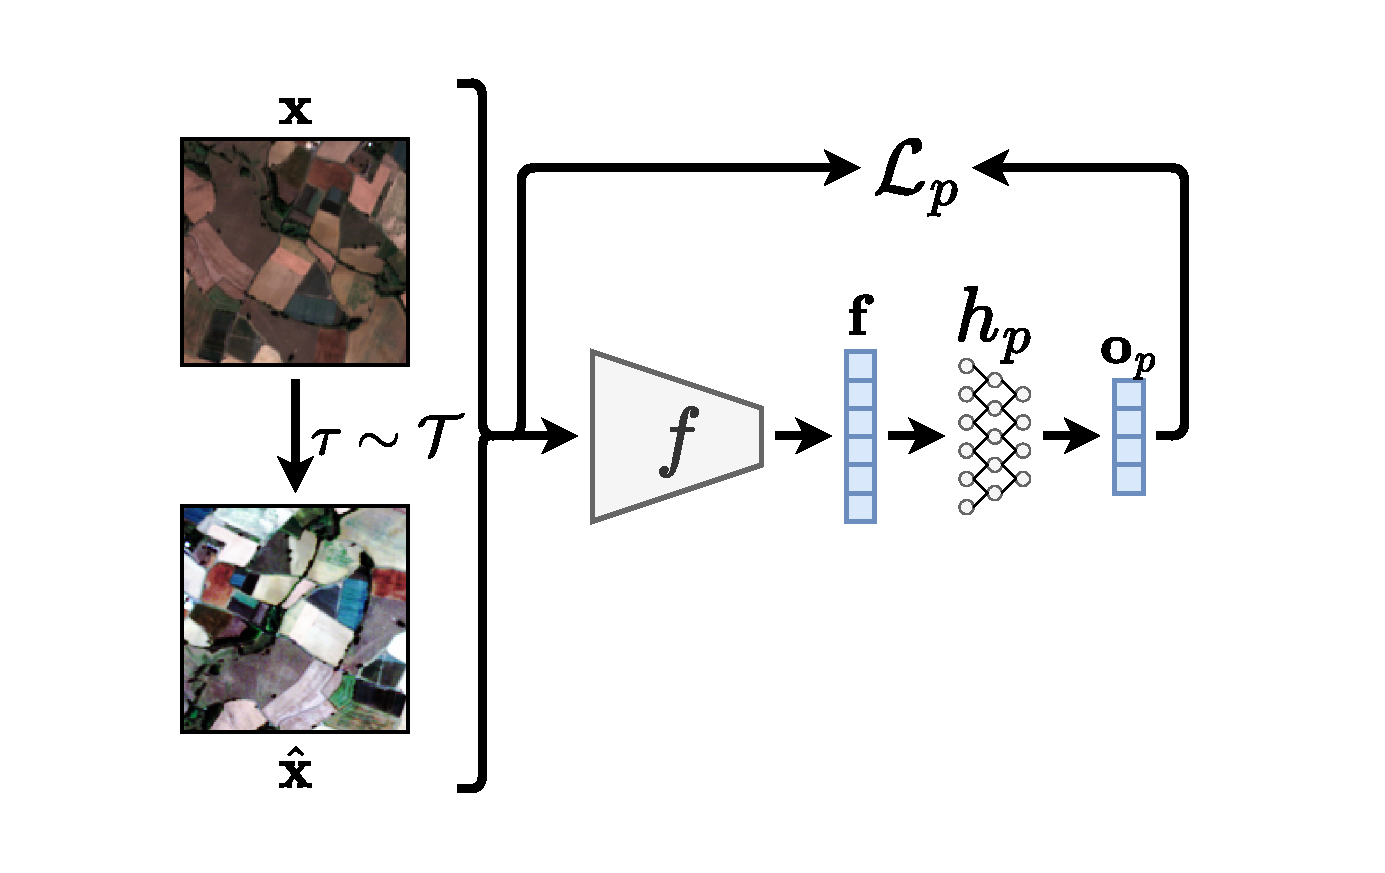
\includegraphics[clip,trim=1.15in 0.45in 0.45in 0.45in,scale=\figscale]{figures/3_theoretical_background/ssl/representation_learning_pre-training.pdf}
        \caption{\fromsurvey{}}
        \label{fig:ssl_overview_pre-training}
    \end{subfigure}
    \\
    \begin{subfigure}[c]{0.975\columnwidth}
        \centering
        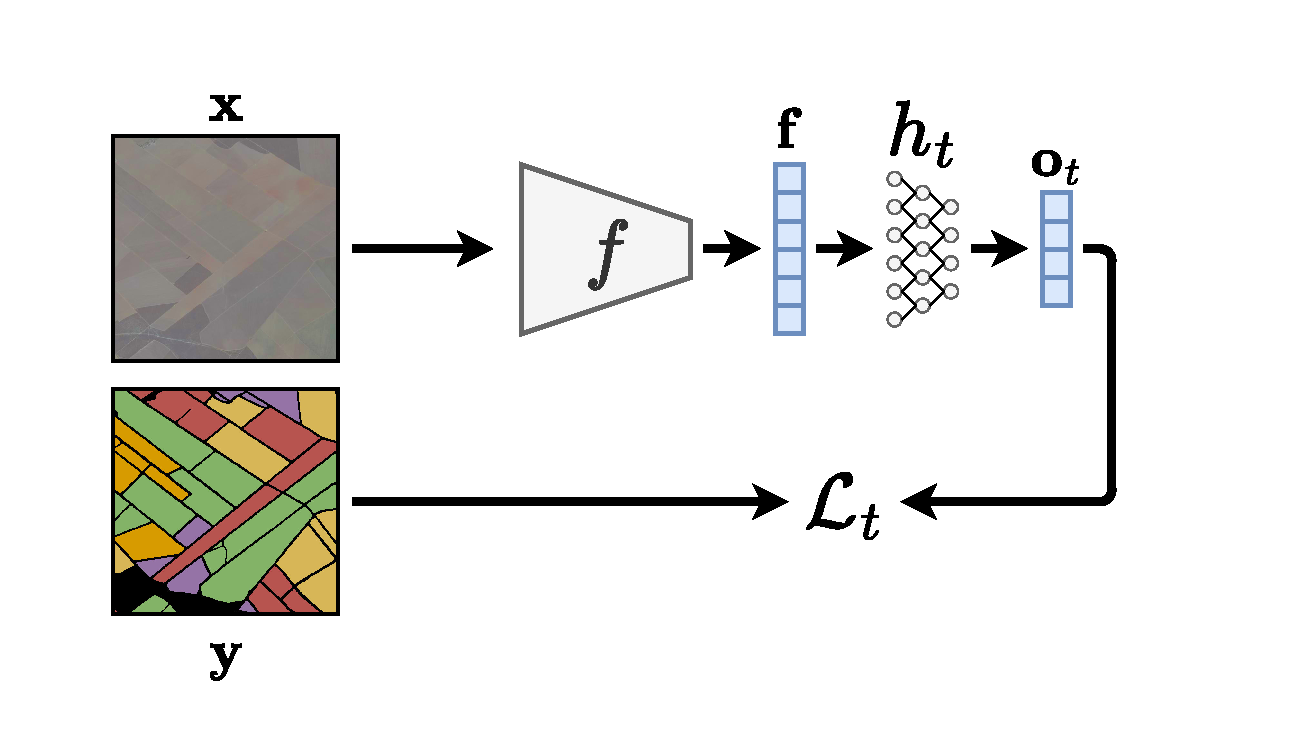
\includegraphics[clip,trim=0.75in 0.45in 0.45in 0.45in,scale=\figscale]{figures/3_theoretical_background/ssl/representation_learning_finetuning.pdf}
        \caption{\fromsurvey{}}
        \label{fig:ssl_overview_finetuning}
    \end{subfigure}
    \fignote{Overview of the self-supervised pretraining process (a) of a model $f$ using a loss $\mathcal{L}_p$ (a), followed by a fine-tuning step (b) to a target labeled task via a loss $\mathcal{L}_t$ (b). One should notice that only the backbone $f$ is maintained, while the pretraining head $h_p$ is swapped for a novel, randomly initialized target task head $h_t$.}
    \label{fig:ssl_overview}
\end{figure}

\fromsurvey{Visual \ac{SSL} began with transform prediction, i.e., procedurally augment an image using geometric, color, or masking transforms and train a model to predict which transform parameter was applied to that image. More formally, given an image $\mathbf{x}$, one can apply a randomly sampled transform $\tau \sim \mathcal{T}$ to generate the transformed version $\hat{\mathbf{x}}$. $\hat{\mathbf{x}}$ can then be passed forwarded through a backbone model $f$, yielding feature vector $\mathbf{f}$. The backbone $f$ and head $h$ are, therefore, trained to predict which randomly sampled transformation $\tau$ was applied to $\mathbf{x}$. For instance, classifying which rotation \citep{gidaris2018unsupervised} or affine transform \citep{kanazawa2016warpnet} a given image underwent. Some tasks not commonly used as data augmentations were also used, like jigsaws on the image, and the pretext task was to classify the correct order for the reconstruction of the original image \citep{kanazawa2016warpnet}. A prototypical transform prediction \ac{SSL} approach can be seen in Figure \ref{fig:ssl_transform}.}

\begin{figure}[ht!]
    \centering
    \caption{Overview of transform prediction self-supervised learning}
    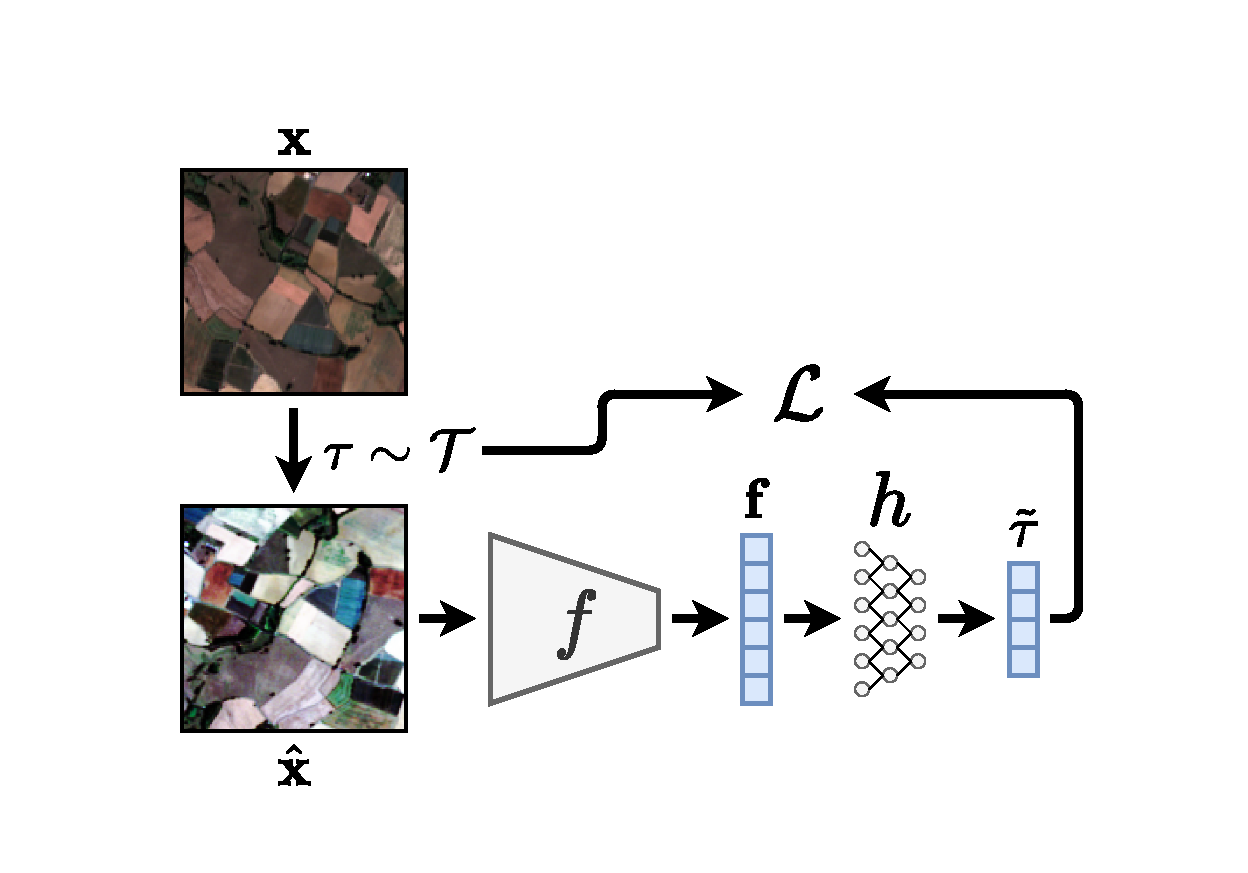
\includegraphics[clip,trim=0.75in 0.45in 0.45in 0.45in,scale=\figscale]{figures/3_theoretical_background/ssl/transform_prediction.pdf}
    \fignote{The original image $\mathbf{x}$ is transformed using $\tau \sim \mathcal{T}$ into $\hat{\mathbf{x}}$, which is fed through the networks $f$ and $h$ to predict $\tilde{\tau}$. A classification or regression loss $\mathcal{L}$ is then used to enforce that $\tilde{\tau} \approx \tau$.}
    \label{fig:ssl_transform}
\end{figure}

\fromsurvey{Little work has been done on transform prediction for \ac{RS}. \cite{wen2021rotation} used rotation prediction for object recognition using \ac{SAR} data, improving few-shot recognition performance. Again, \cite{xu2021self} employed the same methodology for object recognition for optical data. The latter also notes that doing this during semi-supervised hybrid training (see more in Section \ref{sec:ssl_semi}) presents slightly better results.}

\subsection{Similarity-based Self-Supervision}
\label{sec:ssl_similarity}

\fromsurvey{However, transform prediction \ac{SSL} has severe limitations, such as generating covariant embeddings with respect to the transformations applied to the input, as well as unrepresentative representations caused by the backbone learning to identify shortcuts instead of relevant features \citep{minderer2020automatic}. 
In order to extract more representative representations, \ac{SSL} has migrated to similarity-based techniques. Such methods approximate embeddings for multiple views of a single image, rendering the backbones invariant to these data augmentations instead of covariant to them. By doing this, the pretraining procedure encourages the representation to discriminate across instances, generating more sparse embeddings.}


\fromsurvey{Figure \ref{fig:ssl_sim} depicts a similarity-based \ac{SSL} strategy. From a single image $\mathbf{x}$, two views $\mathbf{x}_1 = \tau_1(\mathbf{x})$ and $\mathbf{x}_2 = \tau_2(\mathbf{x})$ are generated by applying two randomly sampled transformations $\tau_1, \tau_2 \sim \mathcal{T}$. $\mathbf{x}_1$ and $\mathbf{x}_2$ are then passed through a backbone $f$, yielding the feature representations $\mathbf{f}_1$ and $\mathbf{f}_2$, which are then passed through a projection head $h$, resulting in the projected vectors $\mathbf{p}_1$ and $\mathbf{p}_2$. The whole ensemble is then trained by encouraging similarity between $\mathbf{p}_1$ and $\mathbf{p}_2$ via a similarity loss $\mathcal{L}_{sim}$.}


\begin{figure}[ht!]
    \centering
    \caption{Overview of similarity self-supervised pretraining.}
    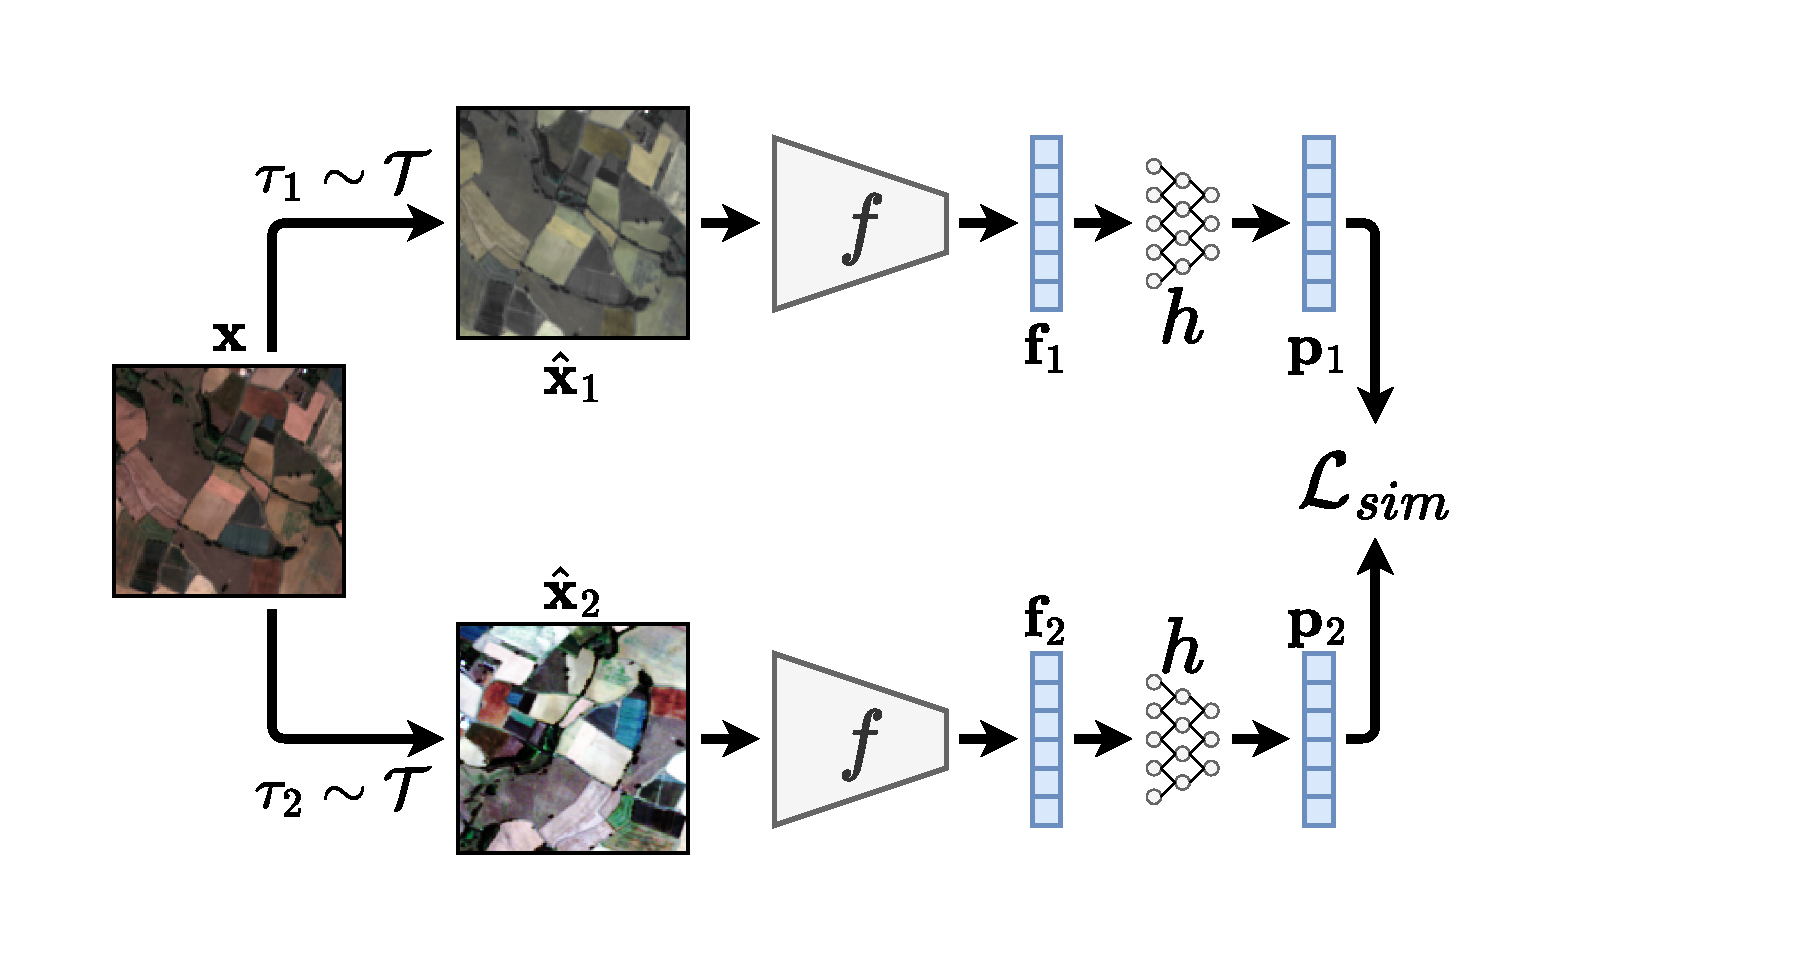
\includegraphics[clip,trim=0.75in 0.45in 2.4in 0.45in,scale=\figscale]{figures/3_theoretical_background/ssl/similarity.pdf}
    \fignote{ Two views $\mathbf{x}_1$ and $\mathbf{x}_2$ from a sample $\mathbf{x}$ computed using the transformations $\tau_1$ and $\tau_2$ are passed through a backbone $f$ and a projection head $h$, yielding projections $\mathbf{f}_1$ and $\mathbf{f}_2$, which are then encouraged to be similar via a similarity loss $\mathcal{L}_{sim}$.}
    \label{fig:ssl_sim}
\end{figure}

\subsubsection{Contrastive Self-Supervised Learning}
\label{sec:ssl_contrastive}

\fromsurvey{In order to avoid the mode collapse problem caused by enforcing similarity between different views of the same image (positive pairs), contrastive \ac{SSL} methods employ very large batch sizes to hold several negative pairs in each learning iteration. Thus, pretraining such contrastive methods may require several \acs{GPU}s with large \ac{VRAM} capacity. \ac{SimCLR} \citep{chen2020simple}, for instance, is a highly influential contrastive \ac{SSL} strategy that requires very large batch sizes. In this approach, the normalized temperature-scaled cross-entropy loss (NT-Xent) is used, leveraging negative pairs from other samples in the batch and achieving a top-1 \ac{OA} of 79.8\% in ImageNet.}

\fromsurvey{Multiple strategies employ smarter ways to leverage negative pairs to avoid the need for large batch sizes. \Acf{MoCo} \citep{he2020momentum, chen2020improved, chen2021empirical} uses a dictionary implemented with a Round Robin queue that stores previously batched negative samples. This makes it possible to decouple the problem of the number of negative pairs from the batch size. In \ac{MoCo}, the key encoder is updated smoothly using a moving average of the query encoder (momentum). This approach leverages the InfoNCE loss to minimize the distance between a query and its positive key and maximize the distance to negative keys, resulting in 81\% in ImageNet in its more recent version.}

\fromsurvey{Another approach to addressing large batch sizes was taken by \cite{caron2020unsupervised} propose \Acf{SwAV} as a pretraining \ac{SSL} strategy. \ac{SwAV} works by predicting online clusters for each augmented multiresolution view of the images via the Sinkhorn-Knopp algorithm. The method does not use direct comparisons between embeddings generated by the augmentations, which eliminates the need for large batch sizes. Instead of traditional instance-wise contrastive learning, \ac{SwAV} is understood as a contrastive clustering approach. As a result, \ac{SwAV} achieved 75.3\% in the same test procedure as \ac{SimCLR} and \ac{MoCo}. \ac{SwAV} was the first \ac{SSL} method to overcome supervised pretraining in ImageNet in transfer learning tasks to other downstream RGB datasets.}

\fromsurvey{Barlow Twins \citep{zbontar2021barlow} use negative samples from the batch itself without the need for a large batch size. This is achieved via a more thorough grid search on the optimizer's hyperparameters. Using a Siamese network that processes two augmented views of the data, Barlow Twins generates a cross-correlation matrix of the augmented embeddings -- twins -- of the batch and trains the network to approximate the identity matrix. By approximating the values of the main diagonal to 1, it forces the invariance of the augmentations. By approximating the other values of the matrix to 0, it avoids collapse. The method has performance comparable to previous methods, including some non-contrastive methods (see Section \ref{sec:ssl_non_contrastive}).}

\fromsurvey{\Acf{SeCo} \citep{yao2021seco} specifically addresses video tasks such as action recognition, untrimmed activity recognition, and object tracking. For this, the models are pretrained on videos, and three pretrained tasks were designed for this: intra-frame discrimination, which determines whether two image patches belong to the same video frame, inter-frame discrimination, which determines whether two image patches belong to the same video, and temporal order validation, which checks whether a sequence of patches is in the correct temporal order. This leads to an improvement in action recognition \ac{OA} of 2.96\% and 6.47\% on UCF101 and HMDB51 against supervised ImageNet pretraining.}

\fromsurvey{Traditional contrastive \ac{SSL} has been employed in RS tasks. \cite{ayush2021geography} adapted \ac{MoCo} by adjusting its augmentations that originally were designed for natural images. For this, temporal views of the same image are used as positive pairs, while images from different positions are used as negative samples. In addition, the prediction of the geolocation of the region of interest is incorporated into the pretext task. For this, the coordinates of the images are previously clustered using K-Means, and the prediction of which cluster each image belongs to is added to the loss. Results indicate that the method outperforms \ac{MoCo} in \ac{RS} tasks. \Acf{DeCUR} \citep{wang2024decoupling} follows the Barlow Twins paradigm, separating inter-modal representations (shared across data modalities) and intra-modal representations (unique within each data modality), enabling the model to learn both shared characteristics and modality-specific features. \ac{DeCUR} outperforms multiple \ac{SSL} methods designed for natural images in both classification and semantic segmentation of images. \ac{SeCo} \citep{yao2021seco} was also used in \ac{RS} \citep{Manas_2021_ICCV} settings, in this case with very few modifications. The results obtained were better in several downstream tasks compared to \ac{MoCo}. These results reinforce the need for domain-specific augmentations in visual \ac{SSL}.}

\subsubsection{Non-Contrastive Self-Supervised Learning}
\label{sec:ssl_non_contrastive}

\fromsurvey{More recently, techniques that do not depend on negative samples have emerged, which completely get rid of the need for memory to store them, either in large batches or in other structures. \Acf{BYOL} \citep{grill2020bootstrap} showed that negative pairs are not needed for avoiding mode collapse. \ac{BYOL} employs two networks: \textit{online} and \textit{target}; wherein the \textit{online} network is trained in a traditional fashion and the \textit{target} is updated with an exponential moving average. The \textit{target} network incorporates a prediction head that projects the embeddings to avoid the collapse of the representations, getting 79.6\% on the same test of \ac{SimCLR}, but using a ResNet with 200 layers. \Acf{DINO} \citep{caron2021emerging} was heavily inspired by \ac{BYOL}, transforming it into a complete knowledge distillation architecture. \ac{BYOL} is heavily focused on optimizing convolutional networks such as ResNet, while \ac{DINO} shows that \acs{ViT}s, show interesting emergent properties of their pretraining. \acs{ViT}s pretrained with \ac{DINO} have internal activations more present in the most informative pixels in the images representing the classes, even with pretraining without labels, achieving 77\% in ImageNet with \acs{ViT}-B/8.}

\fromsurvey{\Acf{SimSiam} \citep{chen2021exploring} considerably simplified non-contrastive \ac{SSL} by approximating embeddings through a Siamese architecture, with one of the branches having an \ac{MLP} as a predictor, and the other applying a stop-gradient operation. The authors describe the method in several ways, including a \ac{SwAV} without online clustering and a \ac{BYOL} without an exponential moving average of the weights, achieving performance very close to contrastive methods. Compared to other non-contrastive methods, \ac{SimSiam} is minimalist, only including what really makes similarity-based \ac{SSL} work without negative pairs. \cite{pototzky2022fastsiam} further improved \ac{SimSiam} into \ac{FastSiam} by regularizing the pretraining by using multiple views instead of only two, achieving similar results, but with only a single \ac{GPU} used during training and a very small batch size.}

\fromsurvey{\cite{bardes2021vicreg} addressed mode collapse in another way, using two forms of regularization in the embeddings: a term that maintains the variance of each embedding dimension above a threshold and a term that decorrelates each pair of variables, creating the \Acf{VICReg} method. \ac{VICReg} does not use negative pairs, while also not using stop-gradient operations, achieving performances comparable to contrastive methods. \Acf{VICRegL} \citep{bardes2022vicregl} builds upon VICReg by adding a new branch to the network responsible for processing local visual information. Even though \ac{VICRegL} results in a 1.1\% drop in classification \ac{OA} in ImageNet, this strategy is shown to be more suited to semantic segmentation and detection tasks. VICRegL yields an 8.1\% mIoU improvement in Pascal VOC, showing that targeted \ac{SSL} pretraining can be better suited to downstream tasks other than image classification.}

\subsection{Masked Modeling}
\label{sec:ssl_mim}

\fromsurvey{Another group of widely used methodologies that draws inspiration directly from \ac{NLP} is \Acf{MM}, in which a portion of the input data for each sample is masked and the pretext task becomes reconstructing the original input data. A typical \ac{MM} approach can be seen in Figure \ref{fig:ssl_mim}. The original image $\mathbf{x}$ is initially sliced into patches, forming the patched image $\mathbf{w}$. A percentage of the patches is masked (hidden), forming $\hat{\mathbf{w}}$, while the masked pixels form the image comprising the invalid pixels $\mathbf{w}_i$. The valid patches are linearized, forming $\hat{\mathbf{w}}_v$ which is passed through the ViT backbone $f$ that serves as an encoder, resulting in the encoded representations $\mathbf{e}_v$. The masked patches are appended to $\mathbf{e}_v$, resulting in $\mathbf{e}_w$, which is passed through the decoder $g$. The output of the ensemble of networks is $\mathbf{d}_w$ representing an embedding with information about the reconstruction of the valid and invalid patches. From $\mathbf{d}_w$, only the originally masked patches are reconstructed in image $\tilde{\mathbf{w}}_i$, which is compared to $\mathbf{w}_i$ via a reconstruction loss $\mathcal{L}_{rec}$.}

\begin{figure}[ht!]
    \centering
    \caption{Overview of masked image self-supervised pretraining.}
    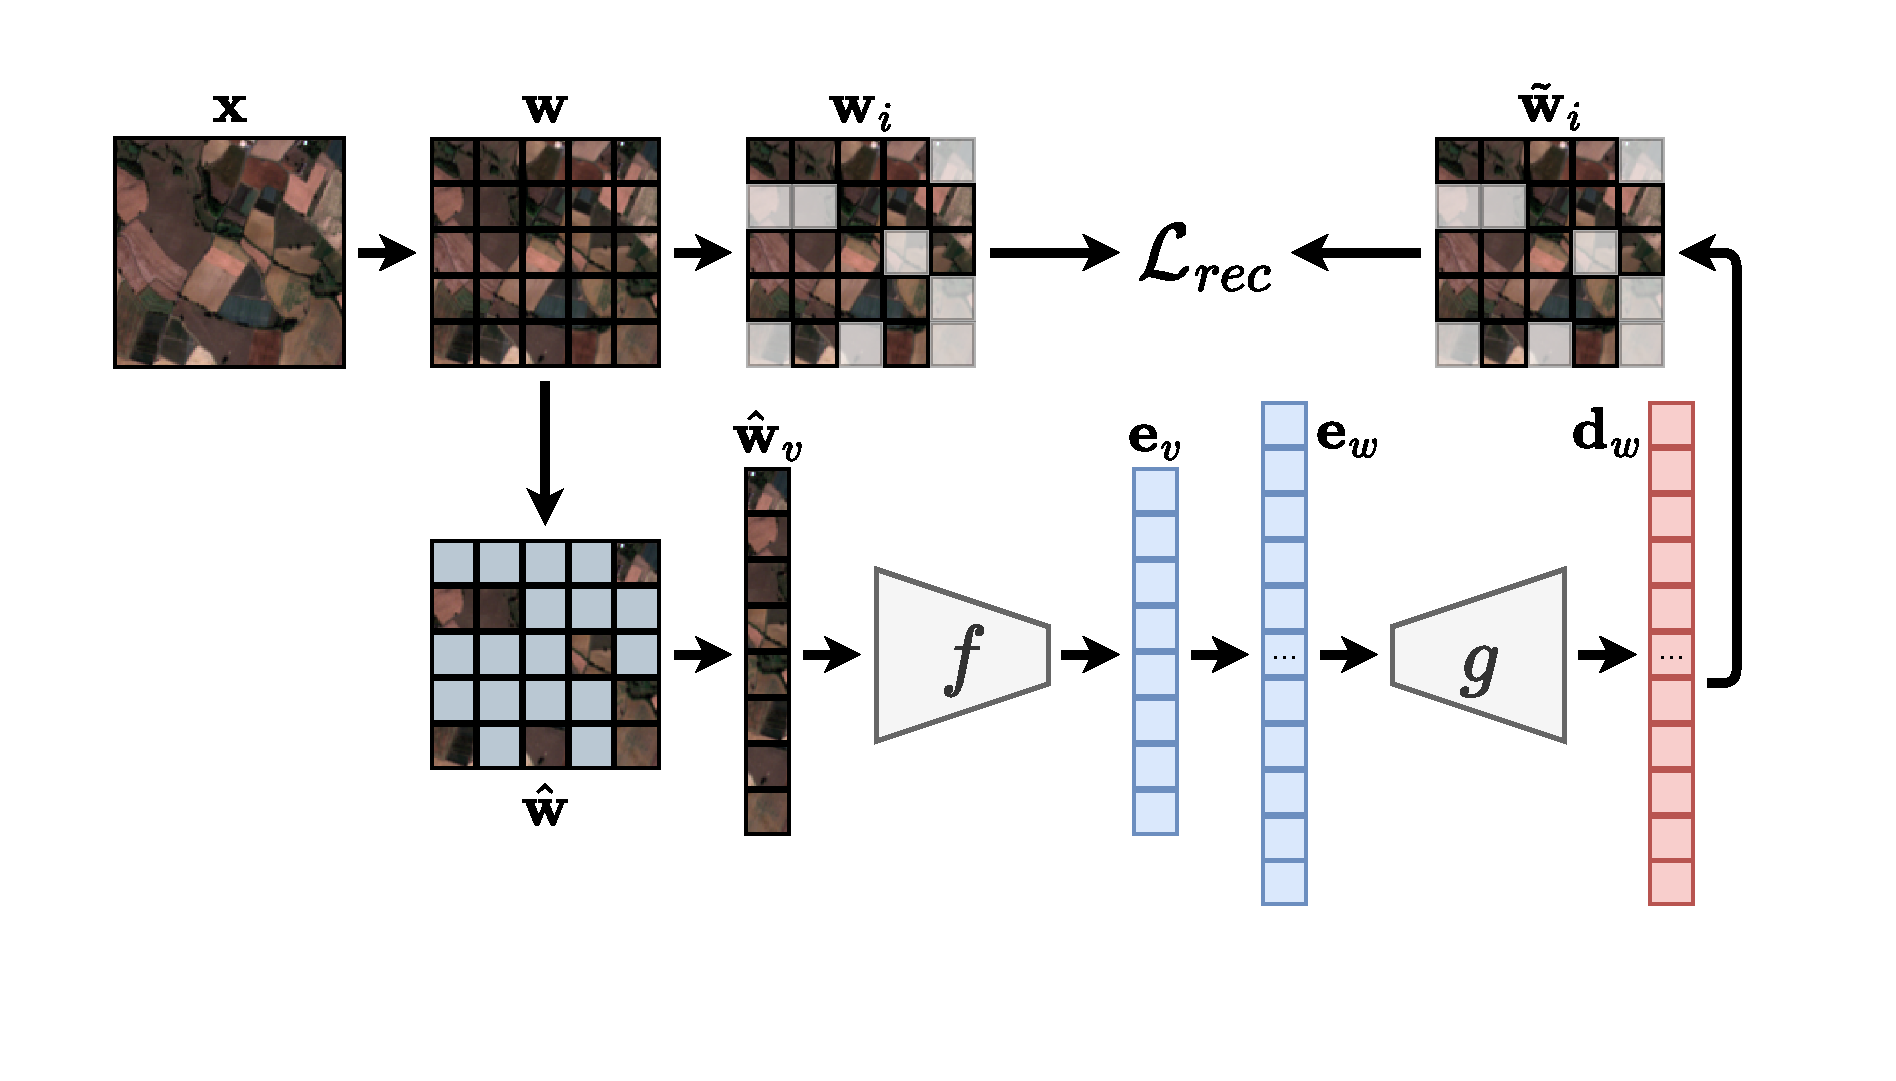
\includegraphics[clip,trim=0.55in 0.4in 0.95in 0.45in,scale=\figscale]{figures/3_theoretical_background/ssl/masked_image_modeling.pdf}
    \fignote{Initially, image $\mathbf{x}$ is windowed, forming $\mathbf{w}$, which yields the valid patch list $\hat{\mathbf{w}}_v$. The patches in $\hat{\mathbf{w}}_v$ are then passed through encoder $f$, resulting in the encoded vector $\mathbf{e}_v$, appended to reinsert the representations of the invalid (masked) patches, resulting in $\mathbf{e}_w$. $\mathbf{e}_w$ is then passed through the decoder $g$, resulting in the reconstruction embedding $\mathbf{d}_w$. From $\mathbf{d}_w$, the reconstruction of the masked patches $\tilde{\mathbf{w}}_i$ is compared to $\mathbf{w}_i$ via a loss $\mathcal{L}_{rec}$. Afterwards, $f$ is repurposed for fine-tuning to a downstream task.}
    \label{fig:ssl_mim}
\end{figure}

\fromsurvey{Following the \ac{MM} paradigm, \Acf{MAE} \citep{he2021maskedautoencodersscalablevision} masks patches from a ViT. The authors showed that the best strategy is to pretrain with 75\% of the patches randomly masked, achieving 76.6\% in ImageNet with a ViT-H/14. Furthermore, it was shown that reconstructing an image without masking patches results in ineffective pretraining, since it is not a complex enough task to force the networks to learn representative features. \Acf{SimMIM} \citep{xie2022simmim} is an approach that works as an advancement and simplification of \ac{MAE}, using direct regression of the RGB values of masked pixels and a lightweight linear decoder head, rendering it a highly efficient pretraining strategy.}

\fromsurvey{Generalist approaches for RS using the idea of data masking have also been developed. \cite{reed2023scale} adapted \ac{MAE} for this domain, introducing a positional encoding based on the spatial resolution of the images. In addition, their Scale-\ac{MAE} separately reconstructs low and high-frequency components using a Laplacian decoder, allowing multiscale learning, while the classic \ac{MAE} reconstructs only the original image. This makes Scale-\ac{MAE} more robust for remote sensing by dealing with multiple scales. The authors demonstrate the improvement in several downstream tasks, including also demonstrating embedding improvement via K-Nearest Neighbors analysis. \cite{xiong2024neural} extended the method based on the idea of neuroplasticity, being able to deal with any number of spectral bands and sensor modalities. Their approach uses a hyper-network-based dynamic weight generator that adjusts its architecture for new sensors, having as input the central reflectance value of each of the bands in addition to the images.}

\fromsurvey{More recent work uses a method that combines MIM with Similarity-based \ac{SSL}, in which views are approximated, but with some having patches of their data masked. Masked Siamese Network (MSN) \citep{assran2022masked} approximates two views of the same image through Negative Cosine Similarity. In the anchor view, some data is masked, while the target view undergoes more aggressive color and geometric augmentations, aiming to render the model invariant to them. Prior Matching for Siamese Networks (PMSN) \citep{assran2022hidden} demonstrated that, although the previous methods do not require pretraining labels, it is still assumed that the classes that exist in the datasets are approximately balanced. To address this, the authors modified the loss function to include a power-law in order to force a balancing of classes per batch, improving the performance on imbalanced data, but degrading the performance on balanced datasets.}

\begin{figure}[ht!]
    \centering
    \caption{\fromsurvey{Overview of masked image similarity self-supervised pretraining.}}
    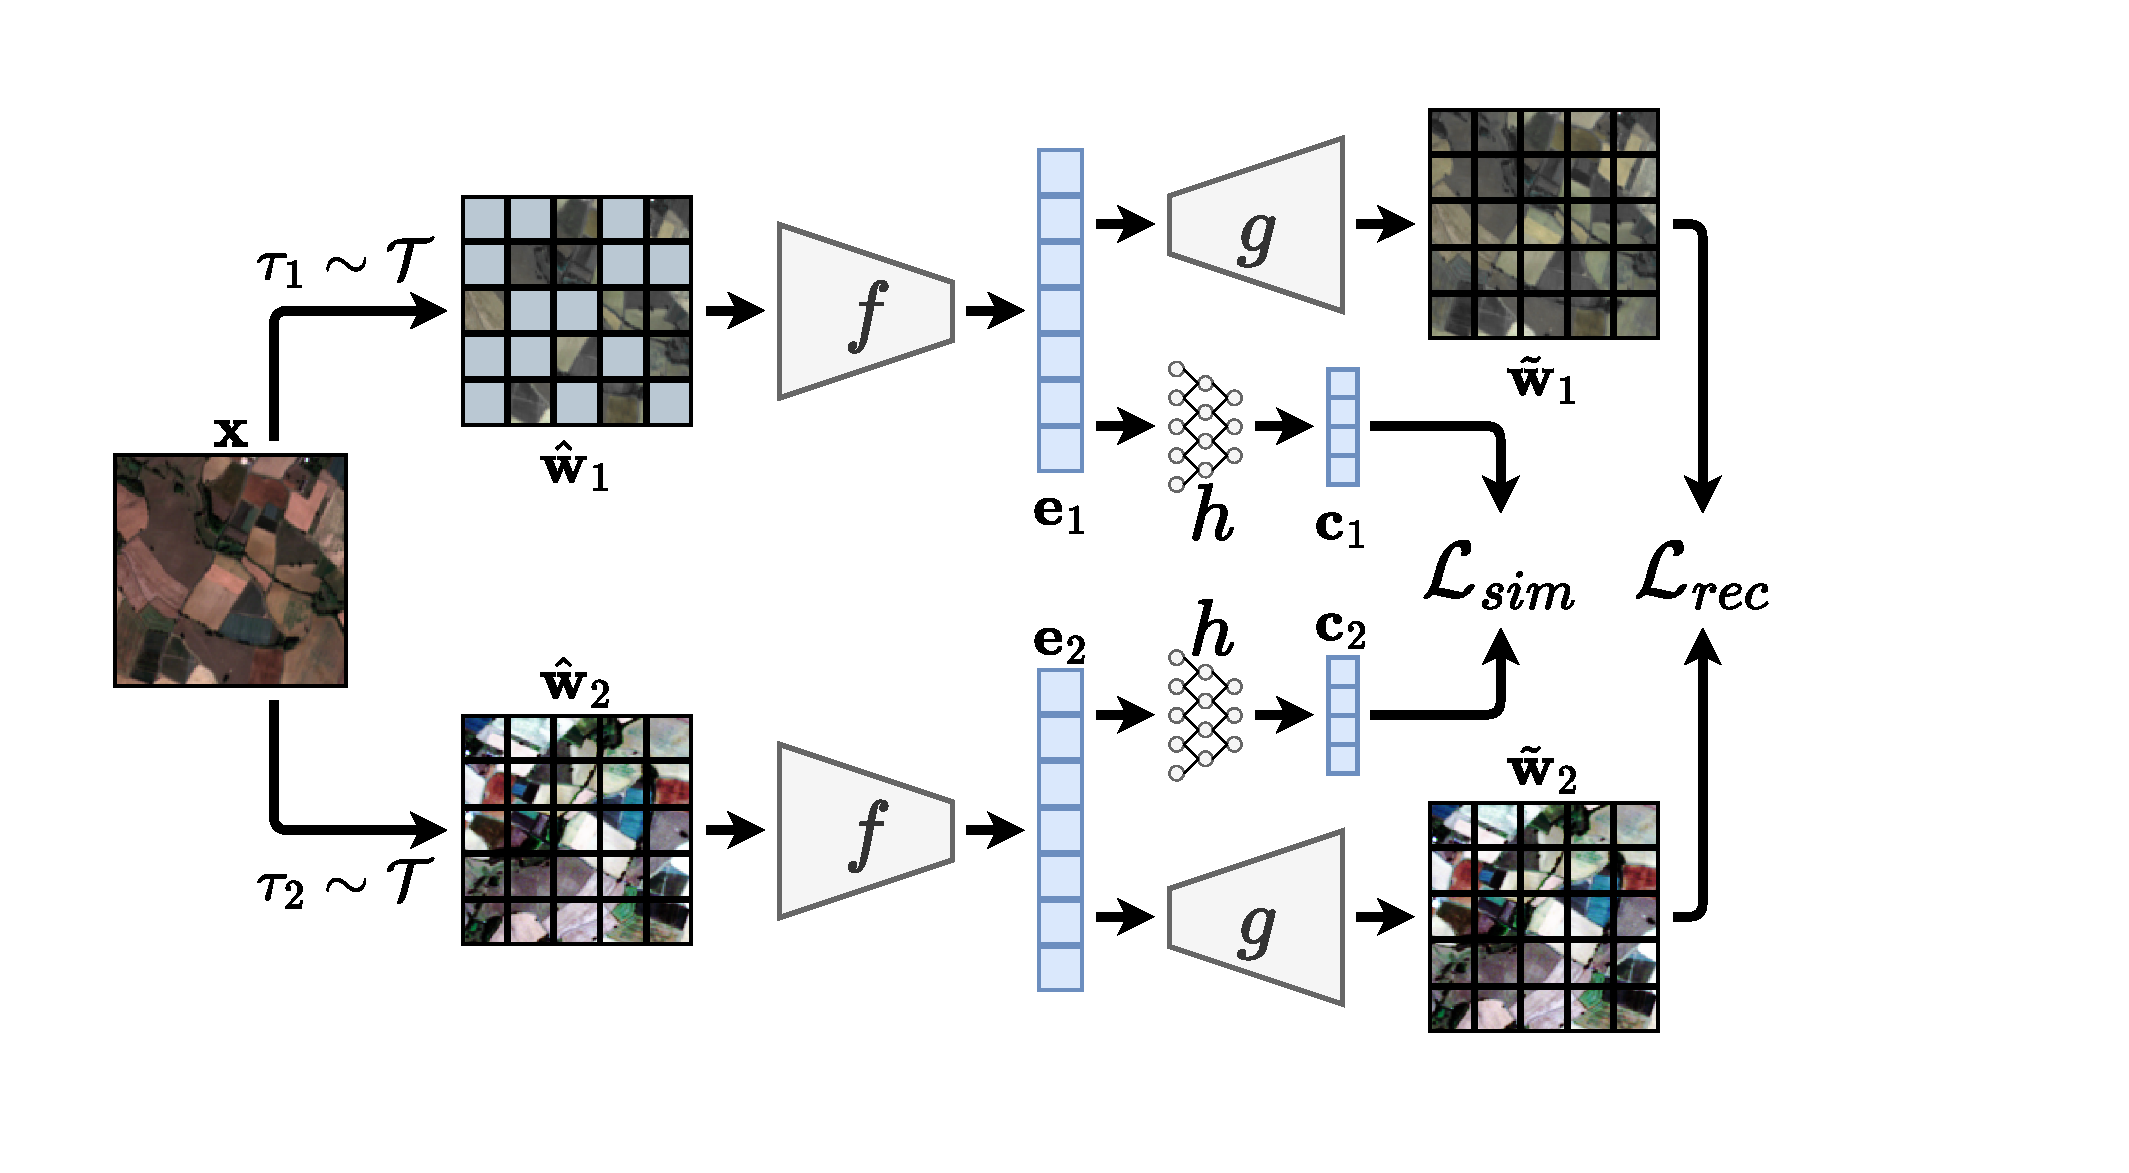
\includegraphics[clip,trim=0.75in 0.45in 2.2in 0.45in,scale=\figscale]{figures/3_theoretical_background/ssl/masked_image_modeling_similarity.pdf}
    \label{fig:ssl_mim_sim}
\end{figure}

\subsection{Semi-Supervised Hybrid Techniques} \label{sec:ssl_semi}

\fromsurvey{A very small area with few published works seeks to combine characteristics of semi-supervised learning with self-supervised learning, based on the hypothesis that \ac{SSL} can benefit from a small number of labeled samples. For this, strategies are used in which the \ac{SSL} pretext task on unlabeled data is performed during finetuning for the downstream task, in a semi-supervised fashion. Following this strategy, \cite{zhai2019s4l} then proposed the \Acf{S4L} method that classifies two augmentations of an image labeled with CELoss, and predicts transforms for these two augmentations added to two more from the unlabeled dataset, achieving the best performance in \ac{OA} on the ILSVRC-2012 Dataset, although comparisons with other methods are lacking. Few methods in this family have been used in \ac{RS}. \cite{singh2018self} used rotation prediction to aid classification, combining the two losses into a so-called Mixup Loss. The results were slightly better using this method, especially considering that rotation prediction in satellite images is quite complex since the directions in the images do not contain much semantic meaning.}